\documentclass{article}
\usepackage{ctex}
\usepackage{enumitem}
\usepackage{siunitx}
\usepackage{graphicx}
\usepackage{amsmath,amsfonts,amsthm}
\begin{document}
\title{高中物理力学辅导}
\author{赵丰 \footnote{Copyright:Creative Commons Attribution-Share Alike 4.0 International}}
\maketitle
\begin{enumerate}
\item \textbf{考虑斜面上一质量为$m$的木块,斜面与水平地面夹角为$\theta$,如图\ref{fig:s}所示,
动摩擦因数为$\mu$,假设木块下滑,求木块沿斜面下滑的加速度$a$。}
\begin{figure}[!ht]
\centering
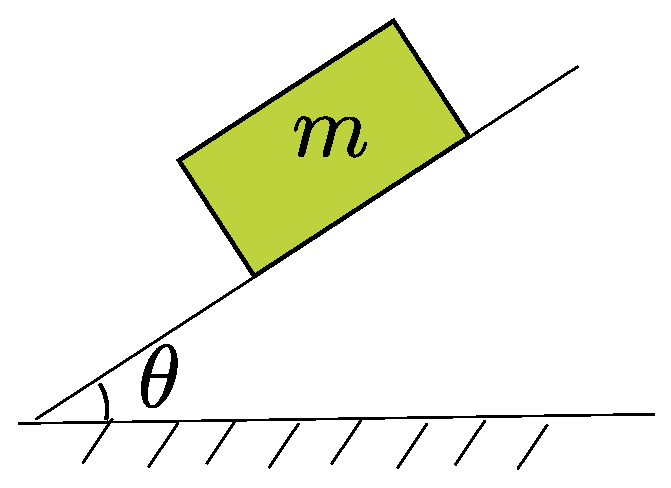
\includegraphics[width=5cm]{fig0.eps}
\caption{斜面上的木块}\label{fig:s}
\end{figure}

由牛顿第二定律可得:
\begin{align}\label{eq:s1}
mg\sin\theta -f =&  ma \\
F_N =& mg\cos\theta \label{eq:s2}
\end{align}
由滑动摩擦因数公式得:
\begin{equation}\label{eq:s3}
f=\mu F_N
\end{equation}
由(\ref{eq:s1},\ref{eq:s2},\ref{eq:s3})解得:
\begin{equation}
a= g(\sin\theta-\mu\cos\theta)
\end{equation}
\textbf{假如施加水平向右的$F$,求$a$。}

由牛顿第二定律可得:
\begin{align}\label{eq:ss1}
mg\sin\theta -f+F\cos\theta =&  ma \\
F_N = & mg\cos\theta + F\sin\theta \label{eq:ss2}
\end{align}
由(\ref{eq:s3},\ref{eq:ss1},\ref{eq:ss2})解得:
\begin{equation}
a= g(\sin\theta-\mu\cos\theta)-\frac{\mu F\sin\theta+F\cos\theta}{m}
\end{equation}

\item \textbf{考虑水平地面一质量为$m$的木块,施加一向下的力$F$,$F$与水平地面夹角为$\theta$,如图\ref{fig:h}所示,动摩擦因数为$\mu$,求木块水平方向的加速度$a$。}
\begin{figure}[!ht]
\centering
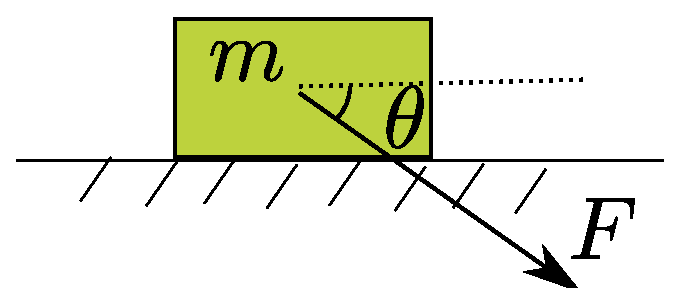
\includegraphics[width=5cm]{fig1.eps}
\caption{水平木块}\label{fig:h}
\end{figure}

由牛顿第二定律可得:
\begin{align}\label{eq:h1}
F\sin\theta + mg =&  F_N \\
F\cos\theta -f =& ma \label{eq:h2}
\end{align}
由(\ref{eq:s3},\ref{eq:h1},\ref{eq:h2})解得:
\begin{equation}
a= \frac{F\cos\theta-\mu F\sin \theta}{m} -\mu g
\end{equation}

\textbf{假如$F$是向上的,与水平方向夹角为$\theta$,求$a$}

\begin{equation}
a= \frac{F\cos\theta+\mu F\sin \theta}{m} -\mu g
\end{equation}

\textbf{$F$向上的,增大到某一个值以上木块会被提起来,求临界的$F$:}
\begin{equation}
F= \frac{mg}{\sin\theta}
\end{equation}
\item \textbf{竖直平面内长为$L$的细绳系着一质量为$m$的小球,从与铅锤方向夹角为$\theta$处静止释放,小球运动过程细绳始终保持拉直状态,求小球运动到最低点时的速度和拉力的大小。}
\begin{figure}[!ht]
\centering
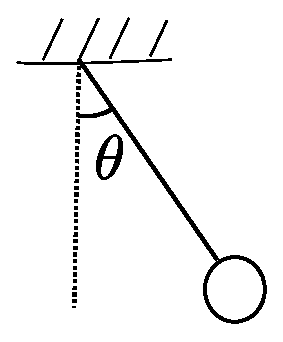
\includegraphics[width=5cm]{fig2.eps}
\caption{}\label{fig:v}
\end{figure}

由动能定理得:
\[
\frac{1}{2}mv^2=mgL\cos\theta
\]
最低点处由牛顿第二定律得:
\[
F_T-mg=\frac{mv^2}{L}
\]
所以$v=\sqrt{2g\cos\theta},F_T=mg(1+2\cos\theta)$
\item \textbf{质量为$m$的小球从高为$h$处水平抛出,初速度为$v_0$,求落地时水平方向的位移。}

由平抛运动的公式
\begin{align*}
h=&\frac{1}{2}gt^2\\
s=&v_0t
\end{align*}
解得:$s=v_0\sqrt{\frac{2h}{g}}$
\item (2016年山东高考物理经典力学18分)如图,一轻弹簧原长为$2R$,其一端固定在倾角为$37^{\circ}$的固定直轨道$AC$的底端$A$处,另一端位于直轨道上$B$处,
弹簧处于自然状态,直轨道与一半径为$\frac{5}{6}R$的光滑圆弧轨道相切于$C$点,$AC=7R,A,B,C,D$均在同一竖直面内。质量为$m$的小物块$P$自$C$点由静止开始下滑,最低到达$E$点,随后$P$沿轨道被弹回,最高点到达$F$点,$AF=4R$,已知$P$与直轨道间的动摩擦因数$\mu = \frac{1}{4}$,重力加速度大小为$g$。(取$\sin37^{\circ}=\frac{3}{5},\cos37^{\circ}=\frac{4}{5}$)
\begin{figure}[!ht]
\centering
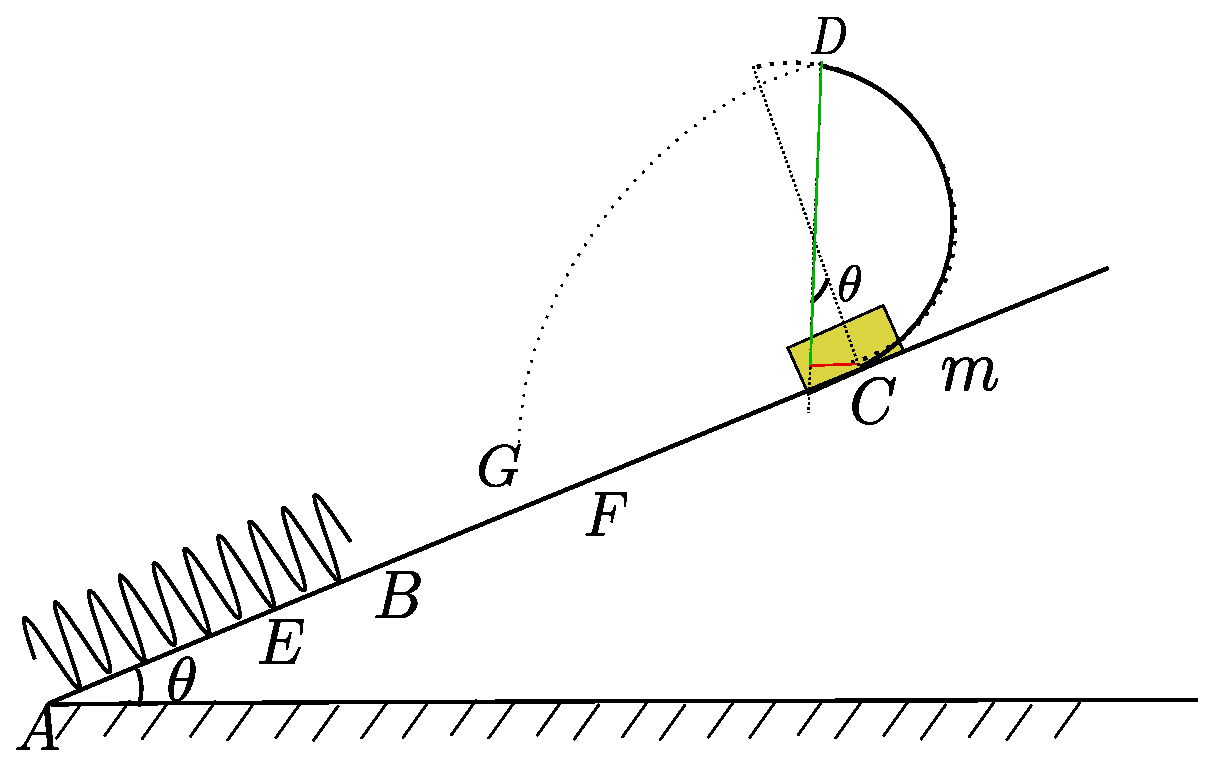
\includegraphics[width=10cm]{2017physics.eps}
\caption{}\label{fig:2017physics}
\end{figure}
\begin{enumerate}[label=(\arabic*)]
\item \textbf{求$P$第一次运动到$B$点时速度的大小}

由动能定理得:
\[
\frac{1}{m}v^2=mg\sin\theta\,CB -mg\cos\theta\,CB
\]
其中$CB=5R$,解得:$v=2\sqrt{gR}$
\item \textbf{求$P$运动到$E$点时弹簧的弹性势能}
\begin{align*}
-\mu mg\cos\theta\, CE+mg\sin\theta \,CE-E_p= &0\\
-\mu mg \cos\theta \, EF-mg\sin\theta\,EF+E_p=& 0
\end{align*}
其中$CE=5R+L,EF=2R+L$
联立上两式解得:$L=R,E_p=\frac{12mgR}{5}$
\item \textbf{改变物块$P$的质量,将$P$推至$E$点,从静止开始释放。已知$P$自圆弧轨道的最高点$D$处水平飞出后,恰好通过$G$点。$G$点在$C$ 点左下方,与$C$点水平相距$\frac{7}{2}R$,竖直相距$R$,求$P$运动到$D$点时速度的大小和改变后$P$的质量。}

由平抛运动的公式
\begin{align*}
\frac{5}{6}R(1+\cos\theta)+R=&\frac{1}{2}gt^2\\
\frac{7R}{2}-\frac{5}{6}R\sin\theta=&v_Dt
\end{align*}
解得:$v_D=\frac{3\sqrt{5gR}}{5}$
\end{enumerate}
从$E$点到$D$点应用动能定理:
\[
\frac{1}{2}Mv_D^2=-Mg h_{ED}-Mg\cos\theta\,CE+E_p
\]
其中$h_{ED}=\sin\theta\,CE+\frac{5}{6}R(1+\cos\theta)$,解得:$M=\frac{m}{3}$
\item \textbf{一质量为$m$的木块以速度$v$在水平面上运动,与一质量为$M$的静止木块发生碰撞,碰撞后两木块以共同的速度$v'$运动,求$v'$。}

由动量守恒定律得:
\[
mv=mv'+Mv'\Rightarrow v'=\frac{mv}{M+m}
\]

该碰撞过程能量的损失是多少?

\[
\frac{1}{2}mv^2-\frac{1}{2}(M+m)v'^2=\frac{M}{2(M+m)}mv^2
\]

\item 如图\ref{fig:2015momentum},三个质量相同的滑块$A,B,C$,间隔相等地静置于同一水平轨道上。现给滑块$A$向右的初速度$v_0$,一段
时间后$A$与$B$发生碰撞,碰后$AB$分别以$\frac{1}{8}v_0,\frac{3}{4}v_0$的速度向右运动,$B$再与$C$发生碰撞,
碰后$B,C$粘在一起向右运动。滑块$A,B$与轨道间的动摩擦因数为同一恒定值。两次碰撞时间极短。求$B,C$碰后瞬间
共同速度的大小。
\begin{figure}[!ht]
\centering
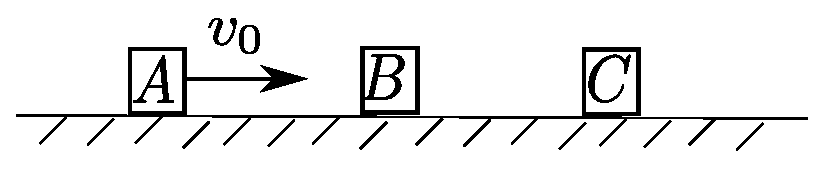
\includegraphics[width=8cm]{2015momentum.eps}
\caption{}\label{fig:2015momentum}
\end{figure}

设$A,B$碰撞前$A$的速度为$v_A,B,C$碰撞前$B$的速度为$v_B$,$B,C$碰后瞬间
共同速度为$v'$,对两次碰撞过程分别应用动量守恒定律:
\begin{align*}
mv_A=& \frac{1}{8}mv_0+\frac{3}{4}mv_0\\
mv_B=& 2mv'\\
\end{align*}
滑块$A$从初始位置到与$B$碰撞的位置,滑块$B$从初始位置到与$C$碰撞的位置两个过程摩擦力做功相等,
对这两个过程分别应用动能定理:
\begin{align*}
\frac{1}{2}mv_A^2-\frac{1}{2}mv_0^2=&W_f\\
\frac{1}{2}mv_B^2-\frac{1}{2}m\left(\frac{3}{4}v_0\right)^2=&W_f
\end{align*}
由以上四个式子解得:$v'=\frac{\sqrt{21}}{16}v_0$
\item 如图\ref{fig:2013momentum}所示,光滑水平轨道上放置以$A$(上表面粗糙)和滑块$C$,滑块$B$置于$A$的
左端。三者质量分别为$m_A=2\si{kg}、m_B=1\si{kg}、m_C=2\si{kg}$。开始时$C$静止,$A,B$一起以$v_0=5m/s$的速度匀速向右运动,
$A$与$C$相碰撞(时间极短)后$C$向右运动,经过一段时间,$A,B$再次达到共同速度一起向右运动,且恰好不再与$C$
碰撞。求$A$与$C$发生碰撞后瞬间$A$的速度大小。
\begin{figure}[!ht]
\centering
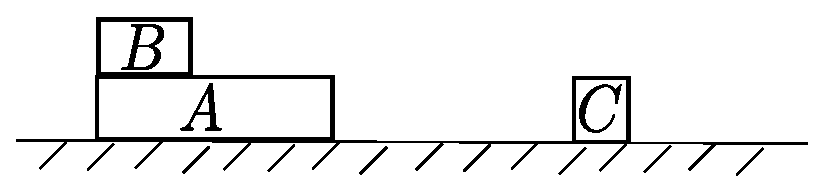
\includegraphics[width=8cm]{2013momentum.eps}
\caption{}\label{fig:2013momentum}
\end{figure}

设$A$和$C$碰撞后速度分别为$v_A$和$v_C$,末状态$v_{A'}=v_{B'}=v_C$,则对$A,C$碰撞过程和$A,B$之间
的摩擦力作用的过程应用动量守恒定律得:
\begin{align*}
m_A v_0 =& m_A v_A + m_C v_C\\
m_Av_A+m_Bv_0 =& (m_A+m_B)v_C
\end{align*}
解得:$v_A=2 \si{m.s^{-1}}$
\end{enumerate}
\end{document}
